\documentclass[acmtog]{acmart}
\usepackage{graphicx}
\usepackage{subfigure}
\usepackage{listings}
\usepackage{color}

\definecolor{mygreen}{rgb}{0,0.6,0}
\definecolor{mygray}{rgb}{0.5,0.5,0.5}
\definecolor{mymauve}{rgb}{0.58,0,0.82}
\lstset{
 backgroundcolor=\color{lightgray}, 
 basicstyle = \footnotesize,       
 breakatwhitespace = false,        
 breaklines = true,                 
 captionpos = b,                    
 commentstyle = \color{mygreen}\bfseries,
 extendedchars = false,             
 frame =shadowbox, 
 framerule=0.5pt,
 keepspaces=true,
 keywordstyle=\color{blue}\bfseries, 
 language = C++,                     
 otherkeywords={string}, 
 numbers=left, 
 numbersep=5pt,
 numberstyle=\tiny\color{mygray},
 rulecolor=\color{black},         
 showspaces=false,  
 showstringspaces=false, 
 showtabs=false,    
 stepnumber=1,         
 stringstyle=\color{mymauve},        
 tabsize=2,          
 title=\lstname                      
}

% Title portion
\title{Assignment 2 : Geometric Modeling} 
\author{Name:\quad Sun Weiliang  \\ student number:\quad 2020533010
	\\email:\quad sunwl1@shanghaitech.edu.cn}

% Document starts
\begin{document}
\maketitle

\vspace*{2 ex}

\section{Outline of the Assignment2}

In this assignment, we are taught to finish several tasks below:

1. Implementation of the basic iterative de Casteljau Bezier vertex evaluation algorithm.

2. Construction of  Bezier Surface with normal evaluation at each mesh vertex.

3. Rendering a Bezier surface in a OpenGL window based on vertex array and vertex normal.

4. Stitching multiple Bezier surface patches together to create a complex meshes.

Bonus part:

1. Adaptive mesh construction in parameter space based on the curvature estimation.

2. B-Spline / NURBS surface construction

3. Interactive editing by selection of control points

4. Cut the Bezier surface with a plane by regenerating the surface mesh according to the cut.

\section{The first task: Implementation of the basic iterative de Casteljau Bezier vertex evaluation algorithm.}

\textbf{1.1 Finish the function evaluate}

In this part, we are asked to finish the function evaluate in the file \textbf{Bezier.cpp}. The function is used to evaluate the Bezier curve at a given parameter value. 

The method to evaluate with a specific value t is to use the iterative de Casteljau algorithm. The algorithm is as follows:

The computation can be expressed recursively. Initially, let $P_{0,j}$ be $P_j$ for j = 0, 1, ..., n. That is, $P_{0,j}$ is the jth entry on column 0. The computation of entry j on column i is the following: 

$$P_{i,j}=(1-t)P_{i-1,j}+tP_{i-1,j+1}$$

To finish this computation:

We have a size to store the size of the control points, and a vector res to store the result which is intialized as the control points.

Then we can know that every step we update each element in the vertex with the formula before.

The special situation is that when it goes into the last step, we need to update the normal by the formula: $normalize(res[1]-res[0])$.

The final return vertex's position is the first element $res[0]$.

\section{The second task: Construction of Bezier Surface with normal evaluation at each mesh vertex.}

\textbf{2.1 Finish the function evaluate (control points, u, v)}

In this part, we should finish the function evaluate with the parameter control points, u and v.

There are two ways to finish this function and the two ways look the same.

The first is to firstly evaluate u and then evaluate v. The second is to firstly evaluate v and then evaluate u.

These two methods get the same result of the position of the vertex. But in the other way, the normal of the vertex is different.

So to get the final normal, I choose to implement two ways of evaluation and get the average.

Getting average doesn't affect the final position of the vertex, but can make the normal more smooth.

\textbf{2.2 Finish the function generateObject()}

We suppose a sample rate num = 50, then at this sample rate to sample the object.

After sampling, we put the vertices and indices into the object's vertices and indices.

One point is arrowed to two triangles which stands for 6 points. So when we read the data, we push back six values in one single loop.

\section{ The third task: Rendering a Bezier surface in a OpenGL window based on vertex array and vertex normal.}

\textbf{3.1 Finish the functions in object.cpp}

The first function in object.cpp is object init:

In this function we init the usual things of OpenGL like VAO, VBO, and EBO.
The implementations are same as assignment1.

The init of the OpenGl can be briefly explained, we import three variables into the code:

1. Vertex Array Object named VAO

2. Vertex Buffer Object named VBO

3. Element Buffer Object named EBO

We need to create a VAO,VBO and EBO to handle the binding procedure. After binding we should import two shader language into the Class Shader, which are named $vertex\_shader.vs$ and $frag\_shader.fs$.(The geometry part will be mentioned in the following bonus part).

\textcolor[rgb]{1,0,0}{\textit{First part--vertex shader:}}

Layout location tells the procedure the location of the vertex attribute. And we also need to claim output which are named $world\_pos$ and $world\_normal$ to get the coordinates in the world space.

In this part we have three important matrixs which are: projection matrix, model matrix and view matrix. After using the three matrixs, we can get the object's world position and world normals in the world space, transmitting the local position and local normal to the world position and world normal. 

The model matrix transform the coordinates into the world space, and the view matrix transform the coordinates into the view space, and the final projection matrix projects the object into a cube.

The formula is as follows:

$$V_{clip}=M_{projection}\cdot M_{view} \cdot M_{model} \cdot V_{local}$$ 

Also we should define the projection matrix and view matrix, which is:

\begin{lstlisting}
	glm::mat4 view = glm::translate(view, glm::vec3(0.0f, 0.0f, -3.0f));
	glm::mat4 projection = glm::perspective(glm::radians(45.0f), Width / Height, 0.1f, 100.0f);
\end{lstlisting}

And then we can use uniform to put these two factors into the vertex shader. Also the function of setMat4() is essential for the transformation from $main.cpp$ to $vertex\_shader.vs$

\textcolor[rgb]{1,0,0}{\textit{Second part--fragment shader:}}

This part include phone lighting same as assignment 1:

In this part, we will do more in fragment shader:

\textcolor[rgb]{1,0,0}{\textit{Setting ambient}}

This is nothing special, like the following code:

\begin{lstlisting}
	float ambient = 0.1;
	vec3 result_color = ambient*light_color*object_color;
	frag_color = vec4(result_color,1.0};
\end{lstlisting}

\textcolor[rgb]{1,0,0}{\textit{Setting diffuse}}

In this part we need to convey the normal from vertex shader to fragment shader. Also we need the light position of the light and the location of the fragment. The world position and world normal can be get from the vertex shader as the above report says.

The first thing we need to calculate is the direction vector between the light source and the fragment's position.The light's direction vector is the difference vector between the light's position vector and the fragment's position vector. So I normalize both the normal and the resulting direction vector:

\begin{lstlisting}
	vec3 normal_direction=normalize(normal);
    vec3 light_direction=normalize(light.position-world_pos); 
    float diffuse=max(dot(normal_direction,light_direction),0.0);
\end{lstlisting}

\textcolor[rgb]{1,0,0}{\textit{Setting specular}}

We negate the lightDir vector. The reflect function expects the first vector to point from the light source towards the fragment's position.We first calculate the dot product between the view direction and the reflect direction and then raise it to the power of 32. This 32 value is the shininess value of the highlight. The higher the shininess value of an object, the more it properly reflects the light instead of scattering it all around and thus the smaller the highlight becomes:

\begin{lstlisting}
	vec3 viewDir = normalize(viewPos - FragPos);
    vec3 reflectDir = reflect(-lightDir, norm);
    float spec = pow(max(dot(viewDir, reflectDir), 0.0), 32);
    vec3 specular = specular * spec * lightColor; 
\end{lstlisting}

And then add them together:

\begin{lstlisting}
	vec3 result = (ambient + diffuse + specular) * objectColor;
    FragColor = vec4(result, 1.0);
\end{lstlisting}

\section{The fourth task: Stitching multiple Bezier surface patches together to create a complex meshes.}

In this part we need to finish the read() function to load the data.

We need to return a vector with element of Bezier surface. We first input the b,p,m,n at the first line.
And then we store all the indices into one single vector with element of vec3. Because of the fact that every
line has n elements, then we set control points at the b line and j*n+k element.

\section{Bonus part: B-Spline / NURBS surface construction.}

In this part, we are taught to do a B-Spline surface instead of the origin Bezier surface.

I create a file named nurbs.hpp which is mainly same as bezier.cpp. But some of the functions changed.

\textbf{1. Degree}

In the b-spline surface we need a new variable named degree. The variable degree means the number of control points
minus 1. In other words, it is described as the highest exponent of the description of the bezier surface.
Its value equals the number of control points minus 1.

\textbf{2. Knot table}

In this part, the second new variable is a table of knots. Knot is a critical variable in b-spline surface, whose size
is strictly the number of control points add degree and 1. The parameters of knot table is set by human beings.

There are two normal ways to set knot table: the first is increasing numbers from 0 to 1. But the first approach has 
disadvantages that it is used to create a close or open b-spline. The second is approach of Clamped. The Clamped approach 
means that we set the first degree+1 points as 0, the last degree+1 points as 1. Between them we divide them fairly to set
the knot table. I use the second method to generate a more smooth and practical b-spline.

\textbf{3. Extra computation of knots}

In this part, the main difference is that we update our control points by knot table.

The main loop is in the function evaluate(). In this function, we use the formula at the most right side
of the tree. And then we use recursion for degree times. By using the formula we get the updated coordinates
and then compute the final b-spline produced points.

\textbf{4. The final result}

To test my b-spline, I create a new bzs file on github named ducky.bzs. Because it is for the test, I only create the body part
of the ducky. In the origin code, when I use bezier surface to create the ducky, the result is as follows:

\begin{figure}[h]
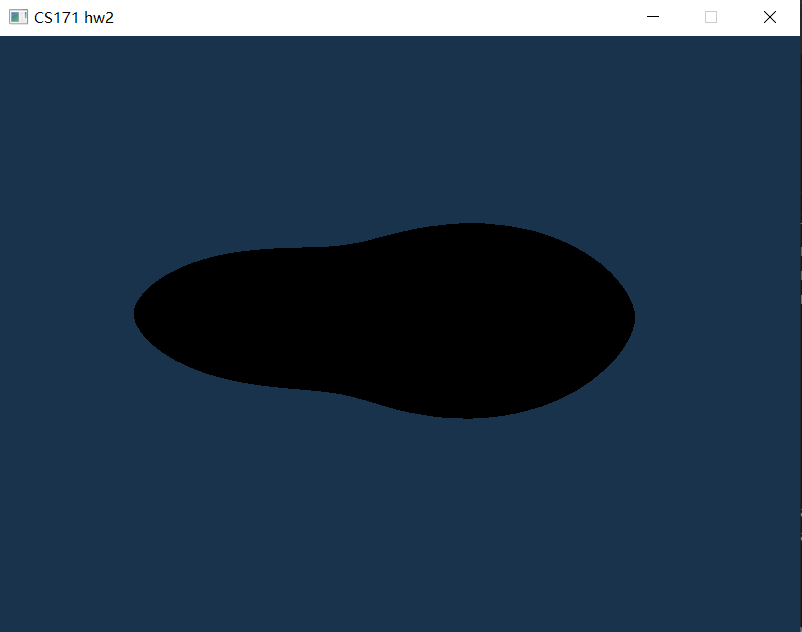
\includegraphics[width=4cm,height=4cm]{origin_ducky}
\caption{the origin result of ducky}
\end{figure}

After the bspline implementation, we can get a new bspline ducky as follows:

\begin{figure}[h]
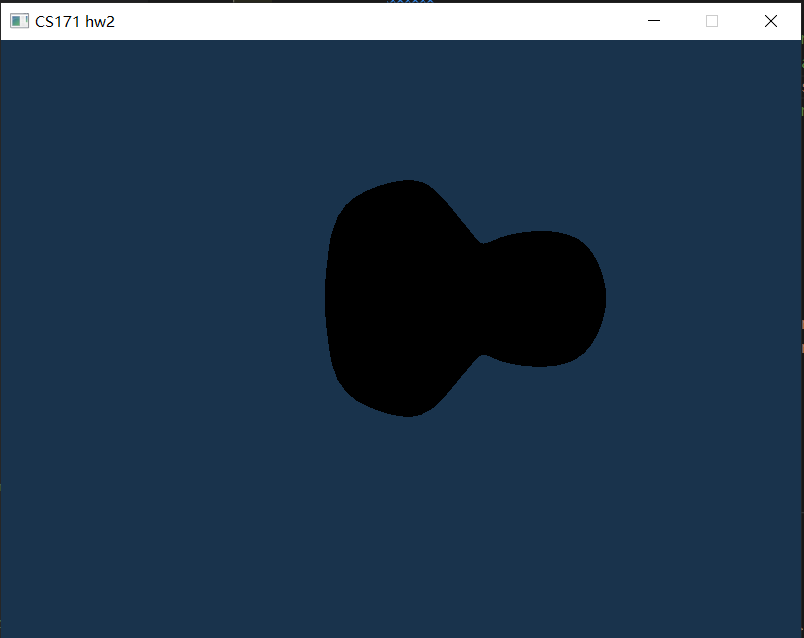
\includegraphics[width=4cm,height=4cm]{bspline_ducky}
\caption{the bspline result of ducky}
\end{figure}

\section{Conclusion}

The final result of the tea is as follows:

\begin{figure}[h]
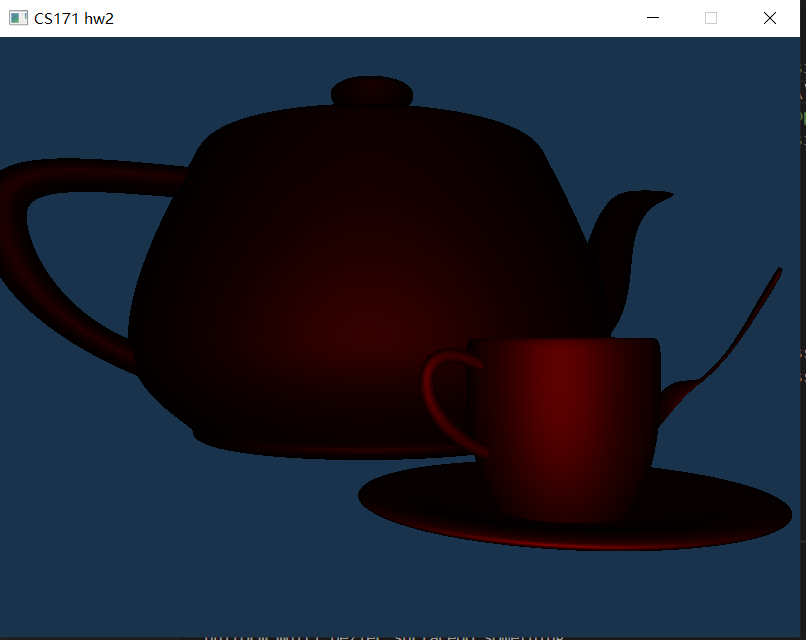
\includegraphics[width=4cm,height=4cm]{final_result}
\caption{the origin result of ducky}
\end{figure}

\end{document}
